\section{The Klein modular invariant function $j$}



\begin{figure}
\centering
\includegraphics[width=0.8\textwidth]{figures/klein-j}
\caption{The composition of the Klein modular invariant function and the inverse modified Cayley transform $j \circ \inv{\ModCayley}$.}
\label{fig_KleinJ}
\end{figure}

\begin{figure}
\centering
\begin{tabular}{c c}
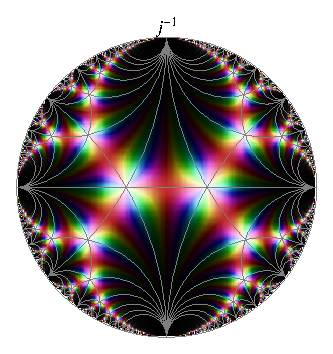
\includegraphics[width=0.4\textwidth]{figures/klein-jinv} &
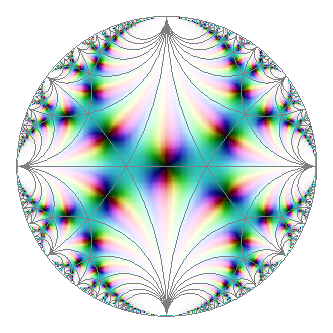
\includegraphics[width=0.4\textwidth]{figures/klein-jm1} \\
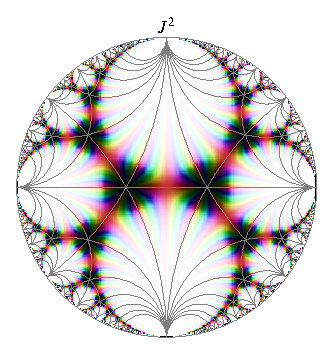
\includegraphics[width=0.4\textwidth]{figures/klein-jsqr} &
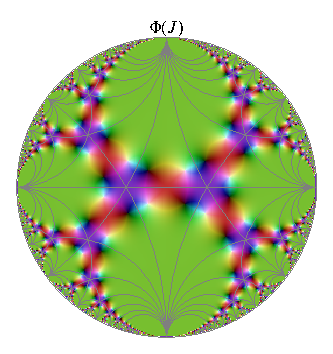
\includegraphics[width=0.4\textwidth]{figures/klein-j-mod-cayley}
\end{tabular}
\caption{The composition of the Klein modular invariant function and the inverse modified Cayley transform $j \circ \inv{\ModCayley}$.}
\label{fig_FunctionsOfJ}
\end{figure}

\begin{figure}
\centering
\includegraphics[width=0.8\textwidth]{figures/klein-jfib-large}
\caption{The composition of the Klein modular invariant function and the inverse modified Cayley transform $j \circ \inv{\ModCayley}$.}
\label{fig_KleinJ_Fib}
\end{figure}
